\documentclass[12pt,a4paper, oneside]{report}

\usepackage[utf8]{inputenc} %Establece codificación a utf8 (para poder escribir tildes)
\usepackage[spanish]{babel} %Traducir títulos a castellano
%Paquetes para f\'ormulas
% \usepackage{amsmath}
% \usepackage{amsfonts}
% \usepackage{amssymb}
%enlaces
\usepackage{url} %Para generar enlaces
\usepackage[breaklinks=true, colorlinks]{hyperref} %Para generar enlaces
%colores
\usepackage{xcolor}
\usepackage{graphicx} %Para trabajar con gráficos
%listados de codigo
\usepackage{listings} %Para listar código fuente
\lstloadlanguages{[LaTeX]TeX}
%Tablas
\usepackage{threeparttable} %Para poner pies de tabla
\usepackage{booktabs} %Para usar toprule, midrule, etc en tablas
\usepackage{subfig} %Para insertar subtablas o subfiguras
\usepackage{multirow} %Para poder usar multicolumn y multirow
\usepackage{colortbl} %Para usar colores en las tablas
% \usepackage{color} %dependencia de colortbl
% \usepackage{array} %dependencia de colortbl
%Otros paquetes
\usepackage{mdwlist} %Define el entorno  basedscript, similar a description
\usepackage{mhchem} %Para escribir fórmulas químicas 
%\chapterstyle{madsen} %Define el estilo de los capítulos de memoir
\author{Digna González Otero}
\title{Información adicional \LaTeX}

\setlength{\parindent}{0cm} %Cambia la indentaci\'on de primera l\'inea
\setlength{\parskip}{8pt} %Cambia la separaci\'on entre p\'arrafos

% Establecemos los valores por defecto de Listings
\lstset{
	language={[LaTeX]TeX},						% Lenguaje por defecto
	%
	% estilos
	keywordstyle=\bfseries\ttfamily\color[rgb]{.8,.1,.2},	% estilos de palabras clave, identificadores, etc...
	identifierstyle=\ttfamily,
	commentstyle=\color[rgb]{0.1,0.5,0.1},			 
	stringstyle=\ttfamily\color[rgb]{0.2,0.2,.7},			
	basicstyle=\footnotesize, 						% the size of the fonts used for the code 
	%
	% numeración (desabilitadas en este momento :-)
	%numbers=left, 								% where to put the line-numbers 
	numberstyle=\footnotesize, 					% size of the fonts used for the line-numbers 
	stepnumber=1, 							% the step between two line-numbers. 
	numbersep=5pt, 							% how far the line-numbers are from the code 
	%
	% espacios
	showspaces=false, 							% show spaces adding particular underscores 
	showstringspaces=false,	 					% underline spaces within strings 
	showtabs=false, 							% show tabs within strings through particular underscores 
	tabsize=6,									% sets default tab-size to 2 spaces
	%
	% cuadro
	backgroundcolor=\color{white}, 				% sets background color (needs package) 
	frame=single, 								% adds a frame around the code
	rulecolor=\color[rgb]{.3,.3,.3},					% set the frame's color. 
	captionpos=b, 								% sets the caption-position to bottom 
	%
	% line breaking
	breaklines=true, 							% sets automatic line breaking 
	breakatwhitespace=false, 					% automatic breaks happen at whitespace 
	prebreak = \raisebox{0ex}[0ex][0ex]{\ensuremath{\hookleftarrow}}, % Nos dibuja una flecha ``guay'' cuando el código no entra en una linea
	escapeinside=@@,		% Para escapar a LaTeX. los acentos
}

\renewcommand*{\contentsname}{Tabla de contenidos}
\renewcommand{\tablename}{Tabla} %Para que se en el caption de las tablas ponga
% Tabla y no Cuadro


\begin{document}
	
	\maketitle
	\newpage
	\tableofcontents
	
\chapter{Información adicional sobre comandos}

\section{Tablas}

Una forma sencilla de crear tablas es usando los entornos \verb+table+, que proporciona un float para insertar tablas, y \verb+tabular+, que genera la propia tabla, como se ha visto en las presentaciones.

Sin embargo, a veces necesitaremos otros comandos y entornos para introducir tablas más avanzadas.

\subsection{Comando \texttt{multicolumn}}

Para escribir texto en una tabla que ocupe varias columnas, usaremos el comando \texttt{multicolumn} que está incluido en el paquete \ \verb+multirow+.
\begin{verbatim}\multicolumn{numColumnas}{alineamiento}{contenido}\end{verbatim}

\begin{lstlisting}
\begin{tabular}{|l|l|}
  \hline
  \multicolumn{2}{|c|}{Team sheet} \\
  \hline
  GK & Paul Robinson \\
  LB & Lucus Radebe \\
  DC & Michael Duberry \\
  \hline
\end{tabular}
\end{lstlisting}

\begin{tabular}{|l|l|}
  \hline
  \multicolumn{2}{|c|}{Team sheet} \\
  \hline
  GK & Paul Robinson \\
  LB & Lucus Radebe \\
  DC & Michael Duberry \\
  \hline
\end{tabular}

\subsection{Comando \texttt{multirow}}

El paquete multirow nos permite construir tablas en que el texto ocupa varias filas. Para ello se utiliza la orden \verb+\multirow+. Esta orden funciona de forma similar a \verb+\multicolumn+, pero para filas.

\begin{verbatim}
\multirow{nrow}{width}[vmove]{contenido}
\end{verbatim}
donde:

\begin{description}
\item [\texttt{nrow}] número de filas a agrupar.
\item [\texttt{width}] Ancho de la columna.
\item [\texttt{vmove}] Sirve para subir o bajar el texto (opcional).
\end{description}

A continuación se muestra una tabla que tiene columnas y filas múltiples usando \verb+multicolumn+ y \verb+\multirow+.

\begin{lstlisting}
\begin{tabular}{|l|l|l|} \hline
\multicolumn{3}{|c|}{Schedulers} \\ \hline
\multirow{3}{*}{Immediate} & RR & Round Robin \\
& EF & Earliest First \\
& LL & Lightest Loaded \\ \hline
\multirow{4}{*}{Batch} & MM & Min-Min \\
& MX & Max-Min \\
& DL & Dynamic Level \\
& RC & Relative Cost \\ \hline
\multirow{4}{*}{Evolutionary} & PN & This paper \\
& ZO & Genetic Algorithm\\
& TA & Tabu search\\
& SA & Simlulated Annealing \\ \hline
\end{tabular}
\end{lstlisting}

\begin{tabular}{|l|l|l|} \hline
\multicolumn{3}{|c|}{Schedulers} \\ \hline
\multirow{3}{*}{Immediate} & RR & Round Robin \\
& EF & Earliest First \\
& LL & Lightest Loaded \\ \hline
\multirow{4}{*}{Batch} & MM & Min-Min \\
& MX & Max-Min \\
& DL & Dynamic Level \\
& RC & Relative Cost \\ \hline
\multirow{4}{*}{Evolutionary} & PN & This paper \\
& ZO & Genetic Algorithm\\
& TA & Tabu search\\
& SA & Simlulated Annealing \\ \hline
\end{tabular}

\clearpage
\subsection{Paquete \texttt{booktabs}}

Para conseguir tablas de aspecto profesional, hay que seguir ciertas reglas de estilo. Algunas de estas reglas son no utilizar nunca líneas verticales ni dobles líneas horizontales.

El paquete \textit{booktabs}\footnote{\url{http://tug.ctan.org/macros/latex/contrib/booktabs/booktabs.pdf}} nos ayuda a dotar a nuestras tablas de un aspecto más profesional, configurando el espaciado entre las líneas y el texto y diferenciando las líneas superior, inferior e intermedias de las tablas.

A continuación se muestra un ejemplo de una tabla generada usando los comandos estándar de LaTeX y la misma tabla generada usando el paquete \textit{booktabs}.

\begin{table}[htb!]
\caption{Comparación entre tablas generadas con y sin \texttt{booktabs}}
\subfloat[Tabla generada con el paquete booktabs \label{tab:ejemploBooktabs}]{
\begin{tabular}[b]{llr} \toprule
\multicolumn{2}{c}{Item} \\ \cmidrule(r){1-2}
Animal & Description & Price (\$)\\ \midrule
Gnat & per gram & 13.65 \\
& each
& 0.01 \\
Gnu
& stuffed
& 92.50 \\
Emu
& stuffed
& 33.33 \\
Armadillo & frozen & 8.99 \\ \bottomrule
\end{tabular}

}
\subfloat[Tabla generada sin el paquete booktabs \label{tab:ejemploNoBooktabs}]
{
\begin{tabular}[b]{@{}llr@{}} \hline
\multicolumn{2}{c}{Item} \\ \cline{1-2}
Animal & Description & Price (\$)\\ \hline
Gnat & per gram & 13.65 \\
& each
& 0.01 \\
Gnu
& stuffed
& 92.50 \\
Emu
& stuffed
& 33.33 \\
Armadillo & frozen & 8.99 \\ \hline
\end{tabular}
}

\end{table}

Como se puede ver, la Tabla \ref{tab:ejemploBooktabs} tiene un aspecto más
legible y agradable, con un mayor espaciado en el encabezado, y con las líneas
superior e inferior destacadas respecto al resto.

El código utilizado para generar esta tabla es el siguiente:

\begin{lstlisting}
\begin{tabular}[b]{llr} \toprule
\multicolumn{2}{c}{Item} \\ \cmidrule(r){1-2}
Animal & Description & Price (\$)\\ \midrule
Gnat & per gram & 13.65 \\
& each
& 0.01 \\
Gnu
& stuffed
& 92.50 \\
Emu
& stuffed
& 33.33 \\
Armadillo & frozen & 8.99 \\ \bottomrule
\end{tabular}
\end{lstlisting}

Los comandos que diferencian a esta tabla de una estándar de \LaTeX{} son los
siguientes:

\begin{description}
\item [\texttt{toprule}] genera la línea superior de la tabla. Se pone justo al
principio.
\item [\texttt{midrule}] línea que delimita el comienzo de los datos de la
tabla.
\item [\texttt{bottomrule}] genera la línea inferior de la tabla.
\item [\texttt{cmidrule}] es el comando análogo a \texttt{cline}, y dibuja una
línea horizontal desde una columna a otra que se le indique.
\end{description}

Además, cargando el paquete \texttt{arrayrulecolor} podemos conseguir tablas con
líneas coloreadas usando el comando \verb+\arrayrulecolor+.

Toda la información sobre el paquete \verb+booktabs+ está en su
documentación\footnote{\url{
http://tug.ctan.org/macros/latex/contrib/booktabs/booktabs.pdf}}.

\clearpage
\subsection{Paquete \texttt{threeparttable}}

El entorno \verb+threeparttable+ soporta la inserción de notas al pie de la
tabla. No es un float, por lo que habría que meterlo dentro de un entorno float
para poder utilizar los \texttt{label} y \texttt{caption}.

\begin{lstlisting}
\begin{table}[htb!]
\begin{threeparttable}[b]
\caption{Tabla generada con threparttable}
\begin{tabular}{l}
Contenido de la tabla\tnote{1}\\
\end{tabular}
\begin{tablenotes}
\item [1] Nota al pie de la tabla
\end{tablenotes}
\end{threeparttable}
\end{table}
\end{lstlisting}

\begin{table}[htb!]
\begin{threeparttable}[b]
\caption{Tabla generada con threparttable}
\begin{tabular}{l}
Contenido de la tabla\tnote{1}\\
\end{tabular}
\begin{tablenotes}
\item [1] Nota al pie de la tabla
\end{tablenotes}
\end{threeparttable}
\end{table}

Como se puede ver en el ejemplo, se ha escrito el comando \verb+\tnote{numero}+
en el lugar donde se quería insertar un número referente al pie de tabla, siendo
número el número a asignar (en este caso la numeración no es automática). Al
final de la tabla, dentro del entorno \verb+tablenotes+ se escriben todas las
notas al pie, siguiendo el formato \verb+\item [numero] Nota+.

Lo habitual será combinar el entorno \verb+\threeparttable+ con el paquete
\verb+booktabs+, como se muestra en el siguiente ejemplo.


\begin{lstlisting}
\begin{table}[htb!]
\begin{threeparttable}[b]
	\begin{tabular}[b]{llr} \toprule
	\multicolumn{2}{c}{Item} \\ \cmidrule(r){1-2}
	Animal & Description & Price (\$)\\ \midrule
	Gnat\tnote{1} & per gram & 13.65 \\
	& each
	& 0.01 \\
	Gnu
	& stuffed
	& 92.50 \\
	Emu
	& stuffed
	& 33.33 \\
	Armadillo & frozen & 8.99 \\ \bottomrule
	\end{tabular}

\begin{tablenotes}
\item [1] Available on demand
\end{tablenotes}
\end{threeparttable}
\end{table}
\end{lstlisting}


\begin{table}[htb!]
\begin{threeparttable}[b]
	\begin{tabular}[b]{llr} \toprule
	\multicolumn{2}{c}{Item} \\ \cmidrule(r){1-2}
	Animal & Description & Price (\$)\\ \midrule
	Gnat\tnote{1} & per gram & 13.65 \\
	& each
	& 0.01 \\
	Gnu
	& stuffed
	& 92.50 \\
	Emu
	& stuffed
	& 33.33 \\
	Armadillo & frozen & 8.99 \\ \bottomrule
	\end{tabular}

\begin{tablenotes}
\item [1] Available on demand
\end{tablenotes}
\end{threeparttable}
\end{table}


\subsection{Uso de colores en tablas}

Para colorear las tablas se utiliza el paquete \verb+\colortbl+.

El documento \url{http://www.tug.org/tutorials/tugindia/chap08-scr.pdf} explica
de forma muy didáctica cómo utilizar colores en tablas.

\clearpage
\subsection{Subtablas y subfiguras}

Se pueden generar varias tablas o figuras que pertenezcan al mismo bloque de
forma que tengan un caption común y también uno independiente, usando el paquete
\verb+subfig+ y el comando \verb+\subfloat+.

La forma de utilizar este entorno es dentro de un entorno float (\verb+figure+ o
\verb+table+), del siguiente modo:

\begin{lstlisting}[numbers=left]
\begin{table}[htb!]
\caption{Caption @común@ a las dos subfiguras}

\subfloat[Texto @índice@ figuras][Texto caption] %
    {\label{etiqueta de la subfigura} %
 Tabla (con \begin{tabular}, etc.)}

\subfloat[Texto @índice@ figuras][Texto caption] %
    {\label{etiqueta de la subfigura} %
 Tabla (con \begin{tabular}, etc.)}
\end{table}
\end{lstlisting}

Como se puede ver en el código, se crea un entorno \verb+table+ que englobará
las dos subfiguras, y se le asigna un caption, que será el caption común de las
dos subfiguras (línea 2). 

A continuación se genera cada subfigura utilizando el comando \verb+subfloat+.
El primer parámetro opcional (entre corchetes) es el texto con que se quiere
que  se referencie la subfigura en el índice de figuras, si lo hubiera. 
Si se ponen los corchetes vacíos, no aparecerá la subfigura en el índice, y
si no se pone  nada (ni siquiera los corchetes), cogerá el texto del caption.

A continuación se pone (también de forma opcional) el caption de la subfigura
entre corchetes. Después, ya entre llaves, se pone el contenido de la tabla en
sí (generado con un entorno tabular), y opcionalmente una etiqueta para hacer
referencia a la subfigura. La etiqueta (label) en realidad se puede poner en
cualquiera de los parámetros que se le pasan al comando. Así, la etiqueta se
podría indicar entre los corchetes del caption, en lugar de dentro de las
llaves.

A continuación se muestra un ejemplo de utilización de este entorno con tablas.

\begin{lstlisting}
\begin{table}[htb!]
\subfloat[][Tabla generada con el paquete booktabs
\label{tab:ejemploBooktabs1}]{
\begin{tabular}{llr} \toprule
\multicolumn{2}{c}{Item} \\ \cmidrule(r){1-2}
Animal & Description & Price (\$)\\ \midrule
Gnat & per gram & 13.65 \\
& each
& 0.01 \\
Gnu
& stuffed
& 92.50 \\
Emu
& stuffed
& 33.33 \\
Armadillo & frozen & 8.99 \\ \bottomrule
\end{tabular}

}
\subfloat[Tabla generada sin el paquete booktabs \label{tab:ejemploNoBooktabs2}]
{
\centering
\begin{tabular}{@{}llr@{}} \hline
\multicolumn{2}{c}{Item} \\ \cline{1-2}
Animal & Description & Price (\$)\\ \hline
Gnat & per gram & 13.65 \\
& each
& 0.01 \\
Gnu
& stuffed
& 92.50 \\
Emu
& stuffed
& 33.33 \\
Armadillo & frozen & 8.99 \\ \hline
\end{tabular}
}
\end{center}
\caption{@Comparación@ entre tablas generadas con y sin \texttt{booktabs}}
\end{table}
\end{lstlisting}

\begin{table}[htb!]
\subfloat[Tabla generada con el paquete booktabs \label{tab:ejemploBooktabs1}]{
\begin{tabular}[b]{llr} \toprule
\multicolumn{2}{c}{Item} \\ \cmidrule(r){1-2}
Animal & Description & Price (\$)\\ \midrule
Gnat & per gram & 13.65 \\
& each
& 0.01 \\
Gnu
& stuffed
& 92.50 \\
Emu
& stuffed
& 33.33 \\
Armadillo & frozen & 8.99 \\ \bottomrule
\end{tabular}

}
\subfloat[Tabla generada sin el paquete booktabs \label{tab:ejemploNoBooktabs2}]
{
\begin{tabular}[b]{@{}llr@{}} \hline
\multicolumn{2}{c}{Item} \\ \cline{1-2}
Animal & Description & Price (\$)\\ \hline
Gnat & per gram & 13.65 \\
& each
& 0.01 \\
Gnu
& stuffed
& 92.50 \\
Emu
& stuffed
& 33.33 \\
Armadillo & frozen & 8.99 \\ \hline
\end{tabular}
}
\caption{Comparación entre tablas generadas con y sin \texttt{booktabs}}
\end{table}

% En este caso las tablas no están perfectamente alineadas porque son de
% diferente tipo. Normalmente, los caption aparecerían siempre alineados.

\clearpage

Bajo estas líneas se muestra otro ejemplo, en este caso con figuras.
% En
% realidad la única diferencia es que se utiliza el comando \verb+subfigure+ en
% lugar de \verb+subtable+. También se utiliza el comando \verb+\hspace+ para
% dejar un espacio horizontal entre las dos figuras.

\begin{lstlisting}
\begin{figure}[htb]
\centering
    \subfloat[Compiladores LaTeX] %
	{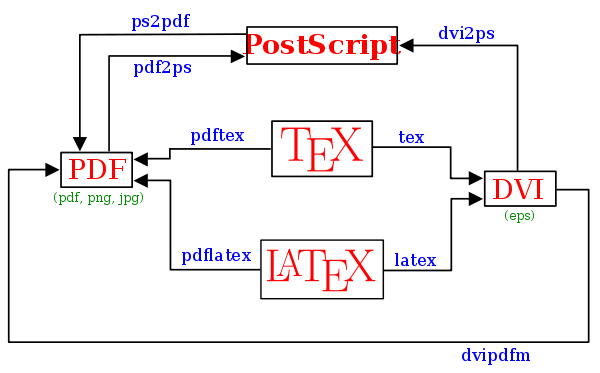
\includegraphics[width=0.4\textwidth]{images/Compiladores.png}}
	\hspace{1cm}
    \subfloat[Comandos]{
      \label{fig:Autenticacion1-b}
      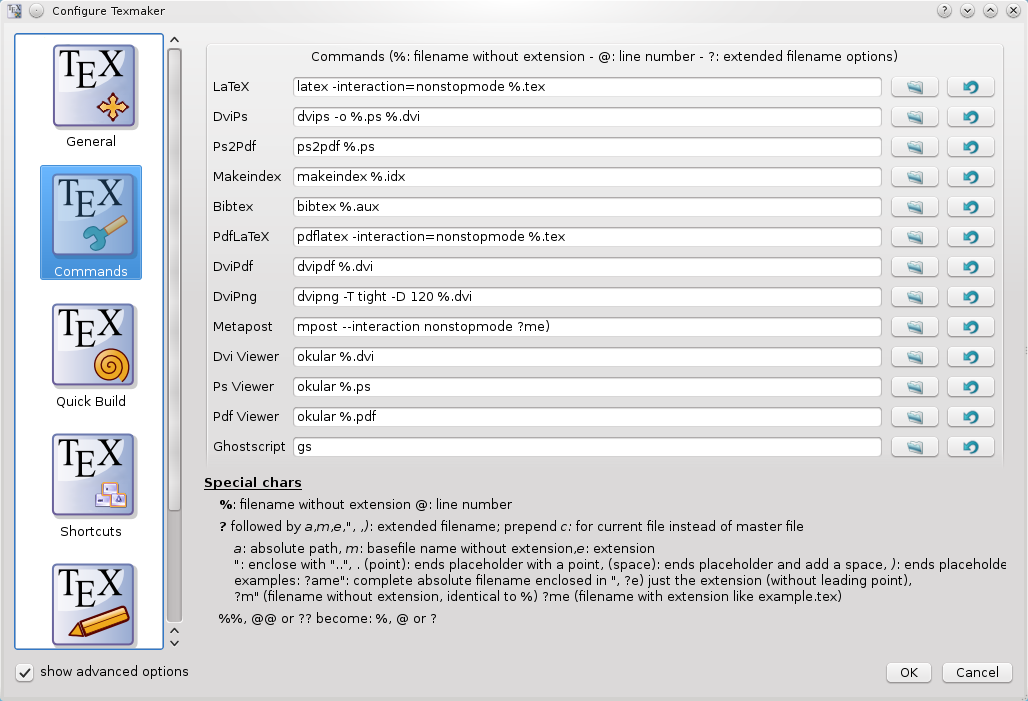
\includegraphics[width=0.4\textwidth]{images/configuracionComandos.png}
    }\\
\caption{@Configuración@ de comandos de LaTeX}
\label{fig:Autenticacion1}
\end{figure}
\end{lstlisting}

\begin{figure}[htb]
        \centering
                \subfloat[Compiladores
LaTeX]{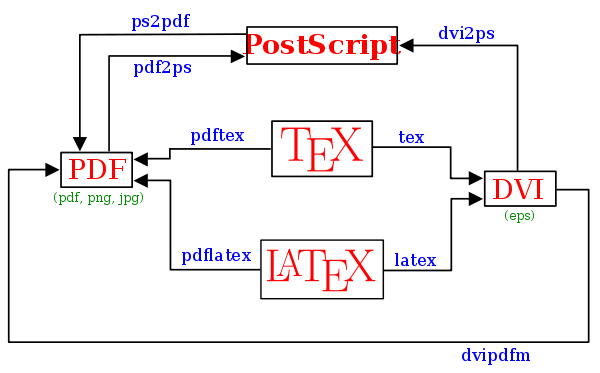
\includegraphics[width=0.4\textwidth]{images/Compiladores.png}}
				\hspace{1cm}
                \subfloat[Comandos]{
                        \label{fig:Autenticacion1-b}
                       
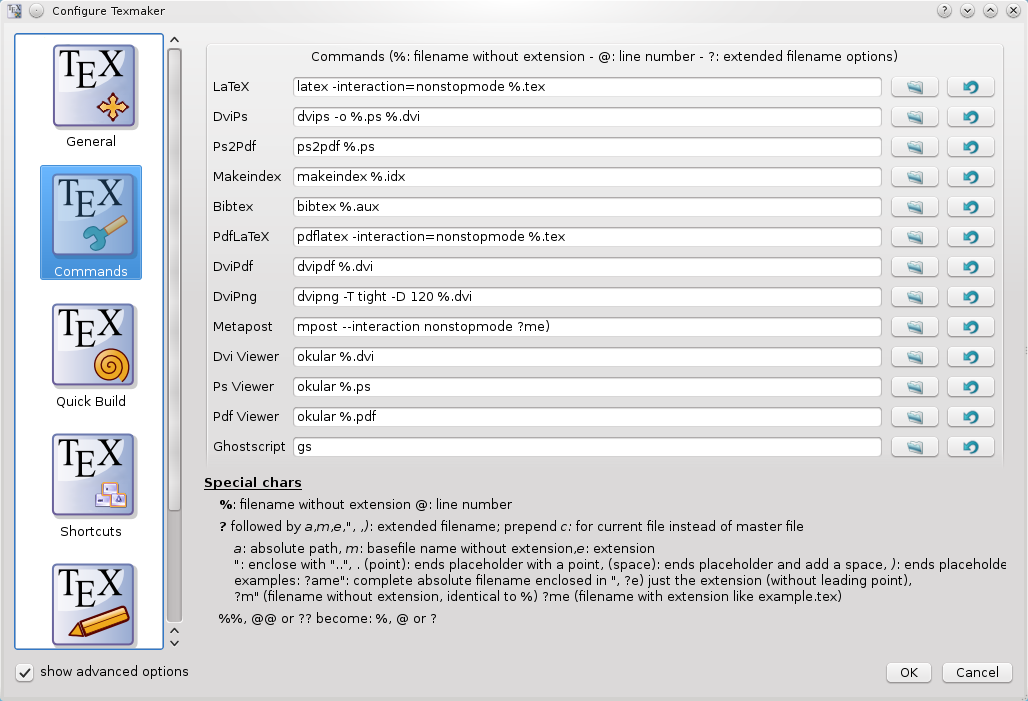
\includegraphics[width=0.4\textwidth]{images/configuracionComandos.png}
                }\\
        \caption{Configuración de comandos de LaTeX}
        \label{fig:Autenticacion1}
\end{figure}

Información y ejemplos en la documentación del
paquete\footnote{\url{http://ctan.org/tex-archive/macros/latex/contrib/subfig/}}
.

\clearpage
\section{Notas al pie}

El comando \texttt{footnote} permite insertar notas al pie\footnote{como en este ejemplo} que se numeran automáticamente. La numeración de las notas al pie se reinicia al empezar un nuevo capítulo (\verb+\chapter{}+), pero es posible reiniciar el contador en cualquier momento usando el comando \verb+\setcounter{footnote}{0}+.

De hecho, cambiando el número que se le pasa como segundo parámetro, se puede asignar cualquier valor al contador.

El comando \verb+\footnotemark{number}+ permite insertar una marca de pie de página con el número que le indiquemos. Es útil para poner un pie de página una vez, y referenciarlo en diferentes puntos del texto\footnotemark[\value{footnote}]. Para que el número se corresponda con el del último pie de página, el comando a utilizar es \verb+\footnotemark[\value{footnote}]+.

El comando \verb+\footnotetext[number]{text}+ incluye cierto texto en el pie de página\footnotetext{como este}, pero no incrementa el contador del pie de página, por lo que, o asignamos un número de forma manual, o mantiene la numeración del último pie de página.

Es muy habitual utilizar simplemente el comando \verb+\footnote{}+ para poner notas al pie, pero también podemos usar \verb+\footnotemark+ y \verb+\footnotetext+ para conseguir notas al pie con la numeración que nosotros decidamos.

\section{Numeración del entorno theorem}

El entorno theorem permite insertar sentencias separadas del texto y con números identificadores. Requiere el paquete \texttt{amsthm}.
\begin{lstlisting}
\newtheorem{midef}{@Definición@}
\begin{midef}
	Esto es una @definición@.
\end{midef}
\end{lstlisting}

Por defecto la numeración de \verb+theorem+ se reinicia al cambiar de capítulo, pero podemos reiniciarlo manualmente usando el comando \verb+\setcounter{midef}{0}+, y sustituyendo \emph{midef} por el nombre del entorno teorema cuyo contador queramos reiniciar.

También es posible que la numeración del teorema haga referencia a la sección o capítulo del texto donde se encuentra. Por ejemplo, ``Teorema 2.3'' haría referencia al tercer teorema del capítulo o sección 2, en función de si estamos en un documento que consta de capítulos o no.

Para conseguir esto, hay que crear el nuevo tipo de teorema con el siguiente comando:

\begin{lstlisting}
\newtheorem{midef}{@Definición@}[numerarPor]
\end{lstlisting}

Siendo \emph{numerarPor} \texttt{chapter}, \texttt{section}, \texttt{subsection}, etc.,en función de la división a la que queremos que haga referencia la numeración. 

\begin{lstlisting}
\newtheorem{midef}{@Definición@}[chapter]
\begin{midef}
	Esto es una @definición@ numerada @según@ el @capítulo@.
\end{midef}
\begin{midef}
	Esto es otra @definición@ numerada @según@ el @capítulo@.
\end{midef}
\end{lstlisting}

\newtheorem{midef}{Definición}[chapter]
\begin{midef}
	Esto es una definición numerada según el capítulo.
\end{midef}
\begin{midef}
	Esto es otra definición numerada según el capítulo.
\end{midef}

\section{Alineación de entorno description}

El entorno \verb+description+ nos permite crear una lista de elementos y su descripción, como en el siguiente ejemplo.

\begin{lstlisting}
\begin{description}
	\item [emph] para enfatizar palabras, de acuerdo al contexto. Recomendado.
	\item [textbf] para texto en \textbf{negrita}.
	\item [textit] para texto en \textit{cursiva}.
	\item [underline] para texto \underline{subrayado}.
	\item [texttt] para texto estilo \texttt{@máquina@ de escribir}.
	\item [textsf] para texto \textsf{Sans-Serif}.
\end{description}
\end{lstlisting}


\begin{description}
	\item [emph] para enfatizar palabras, de acuerdo al contexto. Recomendado.
	\item [textbf] para texto en \textbf{negrita}.
	\item [textit] para texto en \textit{cursiva}.
	\item [underline] para texto \underline{subrayado}.
	\item [texttt] para texto estilo \texttt{máquina de escribir}.
	\item [textsf] para texto \textsf{Sans-Serif}.
\end{description}

Si queremos que en todos los elementos se reserve el mismo espacio para la etiqueta (palabra a describir), de forma que las definiciones empiecen siempre en la misma posición, podemos usar el entorno \verb+basedscript+ contenido en el paquete \verb+mdwlist+

\begin{lstlisting}
\usepackage{mdwlist}
[...]
\begin{basedescript}{\desclabelstyle{\pushlabel}\desclabelwidth{2cm}}
	\item [emph] para enfatizar palabras, de acuerdo al contexto. Recomendado.
	\item [textbf] para texto en \textbf{negrita}.
	\item [textit] para texto en \textit{cursiva}.
	\item [underline] para texto \underline{subrayado}.
	\item [texttt] para texto estilo \texttt{@máquina@ de escribir}.
	\item [textsf] para texto \textsf{Sans-Serif}.
\end{basedescript}
\end{lstlisting}




\begin{basedescript}{\desclabelstyle{\pushlabel}\desclabelwidth{2cm}}
	\item [emph] para enfatizar palabras, de acuerdo al contexto. Recomendado.
	\item [textbf] para texto en \textbf{negrita}.
	\item [textit] para texto en \textit{cursiva}.
	\item [underline] para texto \underline{subrayado}.
	\item [texttt] para texto estilo \texttt{máquina de escribir}.
	\item [textsf] para texto \textsf{Sans-Serif}.
\end{basedescript}

En este caso hay que tener cuidado con dejar espacio suficiente para escribir todas las etiquetas, en caso contrario se podría solapar el texto.

\section{Listando código con lstlistings}

El paquete \verb+listings+ proporciona una forma más configurable de listar código que el entorno \verb+verbatim+.

Para usar este paquete hay que incluirlo en el preámbulo:

\begin{lstlisting}
\usepackage{listings}
\end{lstlisting}

A continuación, para utilizarlo, basta con utilizar el entorno verb+lstlisting+, como en el siguiente ejemplo:

\begin{verbatim}
\begin{lstlisting}
Código a visualizar.
\end{lstlisting}
\end{verbatim}

Sin embargo, para sacar el mayor partido a este comando, es recomendable configurarlo para definir cómo queremos que se muestre el código citado. A continuación se muestra un ejemplo de configuración.

\begin{lstlisting}
\usepackage{listings}
\lstloadlanguages{[LaTeX]TeX}
[...]

% Configuracion de Listings
\lstset{
	language={[LaTeX]TeX},	% Lenguaje por defecto
	% estilos
	keywordstyle=\textbfseries\ttfamily\color[rgb]{.8,.1,.2},	% estilos de palabras clave, identificadores, etc...
	identifierstyle=\ttfamily,
	commentstyle=\color[rgb]{0.1,0.5,0.1},			 
	stringstyle=\ttfamily\color[rgb]{0.2,0.2,.7},			
	basicstyle=\footnotesize, 	% the size of the fonts used for the code 
	% espacios
	showspaces=false, 			% show spaces adding particular underscores 
	showstringspaces=false,	 	% underline spaces within strings 
	showtabs=false, 	% show tabs within strings through particular underscores 
	tabsize=6,			% sets default tab-size to 2 spaces
	% cuadro
	backgroundcolor=\color[RGB]{213,213,255}, 	% sets background color (needs package) 
	frame=single, 								% adds a frame around the code
	rulecolor=\color[rgb]{.3,.3,.3},	% set the frame's color. 
	captionpos=b, 				% sets the caption-position to bottom 
	%
	% line breaking
	breaklines=true, 							% sets automatic line breaking 
	breakatwhitespace=false, 					% automatic breaks happen at whitespace 
	prebreak = \raisebox{0ex}[0ex][0ex]{\ensuremath{\hookleftarrow}}, % Nos dibuja una flecha ``guay'' cuando el @código@ no entra en una linea
	escapeinside=++,		% Para escapar a LaTeX. los acentos
}
\end{lstlisting}

Con esta configuración estamos estableciendo el lenguaje por defecto como \LaTeX{},  configurando el aspecto que queremos que tenga el código mostrado (color de fondo, tipo de texto, etc.). 

Es importante la opción \verb+escapeinside+, que indica qué caracteres tendremos que usar dentro del código para que \LaTeX{} procese lo que hay dentro. Se usa para las tildes, ya que si escribimos tildes directamente, sin poner la palabra que la lleva entre los caracteres de \verb+escapeinside+, obtendremos un error porque \verb+lstlisting+ no está preparado para soportar esa codificación.

Más información sobre este paquete en \footnotesize{ \url{ftp://ftp.tex.ac.uk/tex-archive/macros/latex/contrib/listings/listings.pdf}}.



\section{Protección\protect \footnote{Esto es una prueba para comprobar cómo se pueden poner pies de página en títulos de secciones.} de comandos}

Cuando intentamos hacer ciertas cosas, como poner pies de página en el  nombre de una sección, o una cita en el nombre de una tabla, \LaTeX{} nos da errores. Para solucionarlo tenemos que poner antes del comando problemático el comando \verb+\protect+.

Más información sobre este problema en \url{http://www.tex.ac.uk/cgi-bin/texfaq2html?label=protect}.



\section{Enlaces}

Además de crear enlaces simples incluyendo los paquetes \texttt{url} e \texttt{hyperref} y usando el comando \verb+\url+, también podemos hacer que cierto texto sea un hiperenlace, y al hacer clic sobre él nos lleve a una página web.

Para ello usaremos el comando \verb+\href+, de la siguiente forma: \begin{verbatim}\href{página a enlazar}{texto enlace}\end{verbatim}

Ejemplo: \begin{verbatim}\href{http://www.slideshare.net/digna}{Mi página de slideshare}\end{verbatim} 
El código anterior producirá el siguiente resultado: \href{http://www.slideshare.net/digna}{Mi página de slideshare}

Más información en \href{http://en.wikibooks.org/wiki/LaTeX/Hyperlinks}{la página de Wikibooks de \LaTeX}.


\chapter{Personalización del documento}

\section{Cambiar el título del índice, de los capítulos, etc.}

\LaTeX{} asigna un título a los índices, capítulos, etc, que puede depender del tipo de documento que estemos escribiendo. Por ejemplo, lo que en un artículo se llama \emph{Índice}, en un libro se llama \emph{Índice general}. 

Si no nos gusta la nomenclatura que se utiliza y queremos cambiar alguna de las denominaciones, podemos usar el comando \verb+\renewcommand+.


\begin{verbatim}
\renewcommand{\contentsname}{Contenido}
\renewcommand{\partname}{Parte}
\renewcommand{\indexname}{Lista Alfabética}
\renewcommand{\appendixname}{Apéndice}
\renewcommand{\figurename}{Figura}
\renewcommand{\listfigurename}{Lista de Figuras}
\renewcommand{\tablename}{Tabla}
\renewcommand{\listtablename}{Lista de Tablas}
\renewcommand{\abstractname}{Resumen}
\renewcommand{\chaptername}{Capítulo}
\renewcommand{\refname}{Bibliografía}
\end{verbatim}

En este caso, se ha escrito  justo antes de \verb+\tableofcontents+ la línea \verb+\renewcommand*{\contentsname}{Tabla de contenidos}+. Es decir, hay que introducir el comando justo antes de generar la tabla de contenidos (índice).

\section{Cambiar formato en listas anidadas}

\subsection{Listas numeradas}
Por ejemplo, para que escriba los elementos de primer nivel con números como 1 y los de segundo nivel con números en la forma 1.1

\begin{verbatim}
\renewcommand{\theenumii}{\arabic{enumii}}
\renewcommand{\labelenumii}{\theenumi .\theenumii .}
\end{verbatim}

Si algún paquete que estés usando redefine los \verb+\theenum+, como el babel-spanish, entonces debes asegurate que LaTeX elija tus parámetros colocando las órdenes anteriores entre:

\begin{verbatim}
\AtBeginDocument{%
	comandos aqui..
}
\end{verbatim}

\subsection{Listas no numeradas}
Dentro de un itemize, puede especificarse en cada \verb+\item+  un parámetro opcional, que es el símbolo que se mostrará (en lugar del topo por defecto), por ejemplo, \verb+\item[$\odot$]+, y si se quieren cambiar todos, con el mismo ejemplo,

\begin{verbatim}
\renewcommand{\item}{\item[$\odot$]}
\end{verbatim}

o, mediante el paquete paralist,
\begin{verbatim}
\usepackage{paralist}
...
\begin{itemize}[$\star$]
	\item ...
	\item ...
\end{itemize}
\end{vertabim}

También puede utilizarse el paquete \texttt{pifont}, así:

\begin{verbatim}
\usepackage{pifont}
\begin{Pilist}{pzd}{248}
	\item bla
	\item bla bla
	\item bla
\end{Pilist}
\end{verbatim}

El entorno Pilist es análogo a itemize, pero en lugar del bullet usa el carácter que se le pida de la fuente que se le pida. En el ejemplo anterior, se usa el carácter con código 248 de la fuente pzd que tiene gran cantidad de símbolos adecuados para itemize.


\chapter{Otros truquillos}

\section{Compilación condicional}

\LaTeX{} permite mostrar u ocultar parte del contenido del documento en función del valor de una variable. Esto nos permite, por ejemplo, generar una versión de un examen con soluciones y otra sin ellas con sólo cambiar un valor en el documento y compilar de nuevo, sin tener que tener dos ficheros \texttt{.tex} separados.

Para ello se utiliza el paquete \texttt{ifthen},  y el comando \verb+ifthenelse+, de la siguiente forma:

\begin{lstlisting}
\usepackage{ifthen}
\newboolean{resuelto}
\setboolean{resuelto}{false} % No se muestran las soluciones
[...]

\begin{document}
% Enunciado del ejercicio...
% Ahora vienen las soluciones (se muestran si resuelto es true)
\ifthenelse {\boolean{resuelto}}
{@\texttt{Resolución}@ del ejercicio (texto a escribir en la @\texttt{versión}@ con soluciones)}%
{Texto a escribir en la @versión@ sin soluciones}
\end{lstlisting}
 

\section{Fórmulas químicas}

Las fórmulas químicas sencillas se pueden escribir utilizando la edición de ecuaciones típica de LaTeX. Los subíndices se indican con el caracter \_ y los superíndices con \^. Por ejemplo, el código \verb+$SO_{4}^{2-}$+ genera el siguiente resultado: $SO_{4}^{2-}$.

También se puede utilizar el paquete \texttt{mhchem} para escribir fórmulas químicas de la siguiente forma: \verb+\ce{H2S04}+, obteniendo el siguiente resultado: \ce{H2SO4}. 

Información del paquete en la página \url{http://dante.ctan.org/tex-archive/macros/latex/contrib/mhchem/}.


\ce{6CO2 + 6H2O -> C6H12O6 + 6O2}

\section{Evitar cerrar el pdf cada vez que compilemos}

Si tenemos el pdf abierto con Acrobat Reader  e intentamos compilar, el programa da un error. Podemos utilizar programas alternativos para evitar tener que estar constantemente cerrando el documento. En GNU/Linux los navegadores más utilizados ya hacen eso, pero en Windows podemos instalar por ejemplo Sumatra PDF (software libre y gratuito) de su web\footnote{\url{http://blog.kowalczyk.info/software/sumatrapdf/index.html}}.

También podemos probar sobre Windows aplicaciones de GNU/Linux instalando KDE On Windows\footnote{\url{http://windows.kde.org/}}, que nos permitirá seleccionar qué aplicaciones de Linux queremos instalar. El visor de documentos .ps y .pdf es Okular.



\section{LyX, acercamiento más amigable a \LaTeX}

LyX es un programa libre y multiplataforma (disponible para GNU/Linux, Windows y Mac) que permite escribir documentos \LaTeX{} de forma más sencilla. Proporciona una cierta abstracción respecto a los comandos, es decir, es algo intermedio entre un editor de latex normal, como TexMakerX, y un procesador de textos tradicional: podemos introducir comandos latex, la inclusión de ecuaciones es igual se sencilla y el resultado del documento es muy profesional, pero según escribimos vamos viendo más o menos cómo quedará el documento (no vemos exactamente el resultado final a no ser que compilemos, pero tampoco vemos todos los comandos).

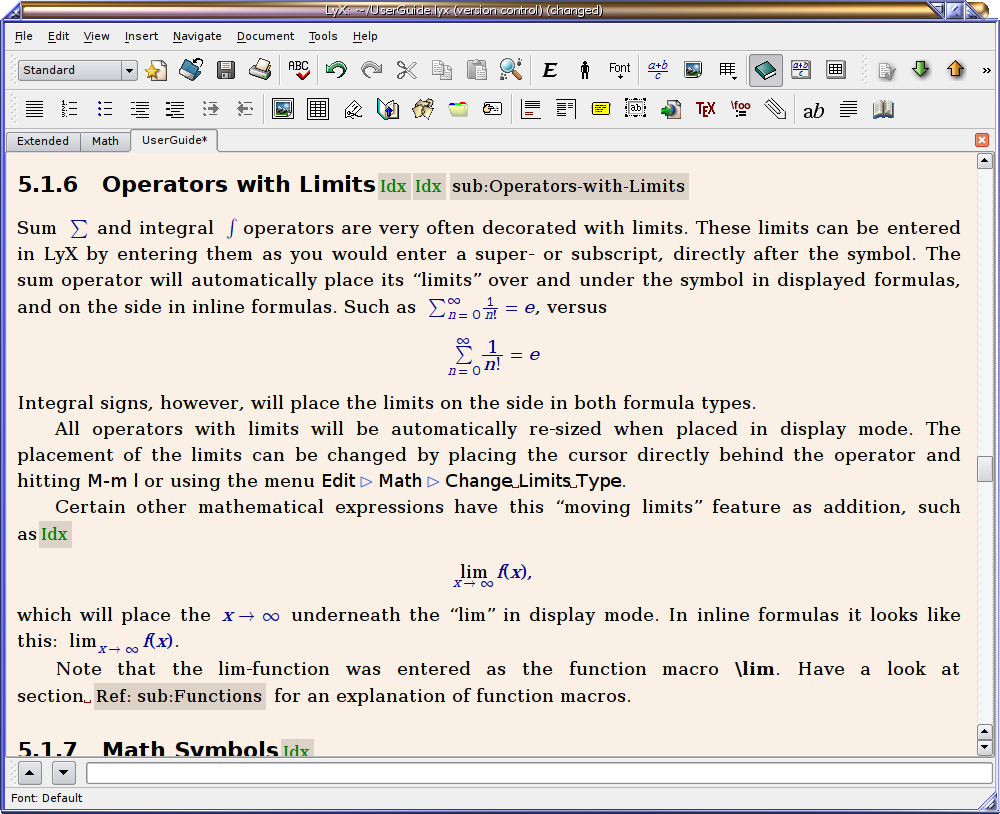
\includegraphics[width=0.9\textwidth]{images/lyx.png}

La forma más sencilla de entenderlo es descargarlo y probarlo, que como es software libre y gratuito no nos cuesta nada. Podemos descargarlo de su web\footnote{\url{http://www.lyx.org/Download}}, donde también encontraremos documentación. Además he marcado en Zotero algunos enlaces útiles con información sobre LyX\footnote{\url{http://www.zotero.org/digna/items/collection/2658205}}.

LyX tiene un tutorial integrado, por lo que para aprender a usarlo recomiendo instalarlo, ir al menú \texttt{Ayuda} y abrir el \texttt{Tutorial}.

\section{Integrar herramientas matemáticas con Lyx}

LyX permite escribir de forma sencilla documentos con fórmulas matemáticas. Si además de escribir estas fórmulas queremos que se procesen y se generen resultados, podemos integrar herramientas matemáticas libres como Máxima, Octave o Maple.

Para ello hay que seguir los siguientes pasos: 

\begin{enumerate}
	\item Descargar e instalar Máxima\footnote{\url{http://maxima.sourceforge.net/download.html}}.
	\item Descargar e instalar LyX\footnote{\url{http://www.lyx.org/Download}}
	\item Reconfigurar LyX: Menú \texttt{Herramientas}, \texttt{Reconfigurar}.
	\item Insertar una ecuación matemática: \texttt{Insertar} $\rightarrow$ \texttt{Ecuación} $\rightarrow$ \texttt{Presentada}.
	\item Menú \texttt{Editar} $\rightarrow$ \texttt{Ecuaciones} $\rightarrow$ \texttt{Usar programa de álgebra} $\rightarrow$ \texttt{Maxima}.
\end{enumerate}

Hay un documento de ejemplo en formato \texttt{.lyx} disponible en \url{http://maxima.sourceforge.net/lyx+maxima.lyx}.

\section{Crear dibujos vectoriales}

Las imágenes vectoriales tienen la ventaja de que no pierden resolución al ser ampliadas. El programa más popular para la creación de imágenes vectoriales es Corel Draw. Sin embargo, existen alternativas libres y gratuitas muy competitivas como \emph{Inkscape}\footnote{\url{http://www.inkscape.org/download/?lang=es}}, que está disponible para varios sistemas operativos.

Otra opción es utilizar el paquete \emph{PSTricks} de \LaTeX{} para dibujar directamente con comandos PostScript.

Para \emph{convertir} imágenes de otros formatos a formato vectorial (\texttt{.eps}), se pueden usar programas de dibujo como Gimp\footnote{\url{http://www.gimp.org/}}, que es libre, gratuito y multiplataforma. 

\end{document}
